\documentclass[12pt]{beamer}\usepackage[]{graphicx}\usepackage[]{color}
%% maxwidth is the original width if it is less than linewidth
%% otherwise use linewidth (to make sure the graphics do not exceed the margin)
\makeatletter
\def\maxwidth{ %
  \ifdim\Gin@nat@width>\linewidth
    \linewidth
  \else
    \Gin@nat@width
  \fi
}
\makeatother

\definecolor{fgcolor}{rgb}{0.345, 0.345, 0.345}
\newcommand{\hlnum}[1]{\textcolor[rgb]{0.686,0.059,0.569}{#1}}%
\newcommand{\hlstr}[1]{\textcolor[rgb]{0.192,0.494,0.8}{#1}}%
\newcommand{\hlcom}[1]{\textcolor[rgb]{0.678,0.584,0.686}{\textit{#1}}}%
\newcommand{\hlopt}[1]{\textcolor[rgb]{0,0,0}{#1}}%
\newcommand{\hlstd}[1]{\textcolor[rgb]{0.345,0.345,0.345}{#1}}%
\newcommand{\hlkwa}[1]{\textcolor[rgb]{0.161,0.373,0.58}{\textbf{#1}}}%
\newcommand{\hlkwb}[1]{\textcolor[rgb]{0.69,0.353,0.396}{#1}}%
\newcommand{\hlkwc}[1]{\textcolor[rgb]{0.333,0.667,0.333}{#1}}%
\newcommand{\hlkwd}[1]{\textcolor[rgb]{0.737,0.353,0.396}{\textbf{#1}}}%
\let\hlipl\hlkwb

\usepackage{framed}
\makeatletter
\newenvironment{kframe}{%
 \def\at@end@of@kframe{}%
 \ifinner\ifhmode%
  \def\at@end@of@kframe{\end{minipage}}%
  \begin{minipage}{\columnwidth}%
 \fi\fi%
 \def\FrameCommand##1{\hskip\@totalleftmargin \hskip-\fboxsep
 \colorbox{shadecolor}{##1}\hskip-\fboxsep
     % There is no \\@totalrightmargin, so:
     \hskip-\linewidth \hskip-\@totalleftmargin \hskip\columnwidth}%
 \MakeFramed {\advance\hsize-\width
   \@totalleftmargin\z@ \linewidth\hsize
   \@setminipage}}%
 {\par\unskip\endMakeFramed%
 \at@end@of@kframe}
\makeatother

\definecolor{shadecolor}{rgb}{.97, .97, .97}
\definecolor{messagecolor}{rgb}{0, 0, 0}
\definecolor{warningcolor}{rgb}{1, 0, 1}
\definecolor{errorcolor}{rgb}{1, 0, 0}
\newenvironment{knitrout}{}{} % an empty environment to be redefined in TeX

\usepackage{alltt}
\usepackage{tikz}

% get rid of junk
\usetheme{default}
\usefonttheme[onlymath]{serif}
\beamertemplatenavigationsymbolsempty

% define a bunch of colors
\definecolor{offwhite}{RGB}{255,250,240}
\definecolor{gray}{RGB}{155,155,155}
\definecolor{foreground}{RGB}{80,80,80}
\definecolor{background}{RGB}{255,255,255}
%\definecolor{title}{RGB}{255,199,0}
\definecolor{title}{RGB}{89,132,212}
%\definecolor{subtitle}{RGB}{89,132,212}
\definecolor{subtitle}{RGB}{255,199,0}
\definecolor{hilit}{RGB}{248,117,79}
\definecolor{vhilit}{RGB}{255,111,207}
\definecolor{lolit}{RGB}{200,200,200}
\definecolor{lit}{RGB}{255,199,0}
\definecolor{mdlit}{RGB}{89,132,212}
\definecolor{link}{RGB}{248,117,79}

% a few color macros
\newcommand{\hilit}{\color{hilit}}
\newcommand{\vhilit}{\color{vhilit}}
\newcommand{\lit}{\color{lit}}
\newcommand{\mdlit}{\color{mdlit}}
\newcommand{\lolit}{\color{lolit}}

% use those colors
\setbeamercolor{titlelike}{fg=title}
\setbeamercolor{subtitle}{fg=subtitle}
\setbeamercolor{frametitle}{fg=gray}
%\setbeamercolor{structure}{fg=subtitle}
\setbeamercolor{structure}{fg=title}
\setbeamercolor{institute}{fg=lolit}
\setbeamercolor{normal text}{fg=foreground,bg=background}
\setbeamertemplate{itemize subitem}{{\textendash}}
\setbeamerfont{itemize/enumerate subbody}{size=\small}
\setbeamerfont{itemize/enumerate subitem}{size=\small}

% center title of slides
\setbeamertemplate{blocks}[rounded]
\setbeamertemplate{frametitle}[default][center]

% page number
\setbeamerfont{page number in foot}{size=\footnotesize}
\setbeamertemplate{footline}[frame number]

% default link color
\hypersetup{colorlinks, urlcolor={link}}

% a few macros
\newcommand{\code}[1]{\texttt{#1}}
\newcommand{\hicode}[1]{{\hilit \texttt{#1}}}
\newcommand{\locode}[1]{{\lolit \texttt{#1}}}
\newcommand{\bb}[1]{\begin{block}{#1}}
\newcommand{\eb}{\end{block}}
\newcommand{\bi}{\begin{itemize}}
\newcommand{\bbi}{\vspace{4pt} \begin{itemize} \itemsep8pt}
\newcommand{\ei}{\end{itemize}}
\newcommand{\bv}{\begin{verbatim}}
\newcommand{\ev}{\end{verbatim}}
\newcommand{\ig}{\includegraphics}
\newcommand{\subt}[1]{{\footnotesize \color{subtitle} {#1}}}
\newcommand{\ttsm}{\tt \small}
\newcommand{\ttfn}{\tt \footnotesize}
\newcommand{\figh}[2]{\centerline{\includegraphics[height=#2\textheight]{#1}}}
\newcommand{\figw}[2]{\centerline{\includegraphics[width=#2\textwidth]{#1}}}



%------------------------------------------------

\title{What is Color?}
\subtitle{Intro to Data Visualization}
\author{\href{http://www.gastonsanchez.com}{Gaston Sanchez}}
\institute{\href{https://creativecommons.org/licenses/by-sa/4.0/}{\tt \scriptsize \color{foreground} CC BY-SA 4.0}}
\date{}
\IfFileExists{upquote.sty}{\usepackage{upquote}}{}
\begin{document}


{
  \setbeamertemplate{footline}{} % no page number here
  \frame{
    \titlepage
  } 
}

%------------------------------------------------

\begin{frame}
\begin{center}
\Huge{\hilit{What is Color?}}
\end{center}
\end{frame}

%------------------------------------------------

\begin{frame}
\frametitle{What is Color?}

\bb{4 ways to talk about color}
One of the difficulties in talking about color is that it seems to exist in
several different forms:
\bbi
  \item material color
  \item radiant color
  \item visual color
  \item conceptual color
 \ei
\eb

\end{frame}

%------------------------------------------------

\begin{frame}
\frametitle{Material Color}
\begin{center}
\ig[width=10cm]{images/material-color.pdf}
\end{center}
\end{frame}

%------------------------------------------------

\begin{frame}
\frametitle{Material Color}

\bb{Material Color}
Material color is the physical pigment, dye, filter, pigmented or dyed 
material, or light source that originates the experience of color. It is the
sense in which we equate color with the physical world.
\eb

{\lolit {\small Bruce MacEvoy}}

\end{frame}

%------------------------------------------------

\begin{frame}
\frametitle{Radiant Color}
\begin{center}
\ig[height=8cm]{images/radiant-color.pdf}
\end{center}
\end{frame}

%------------------------------------------------

\begin{frame}
\frametitle{Radiant Color}

\bb{Radiant Color}
Radiant color is the mixture of light wavelengths emitted by a light 
source, or transmitted by a filter or other semitransparent medium, or 
reflected from an opaque material such as paint, ink, dye, or photographic 
emulsion. This defines color as a physical stimulus.
\eb

{\lolit {\small Bruce MacEvoy}}

\end{frame}

%------------------------------------------------

\begin{frame}
\frametitle{Visual Color}
\begin{center}
\ig[height=8cm]{images/c3po.pdf}
\end{center}
\end{frame}

%------------------------------------------------

\begin{frame}
\frametitle{Visual Color}

\bb{Visual Color}
Visual color is the perception of radiant color in a specific viewing 
context. Visual color literally does not exist outside individual consciousness.
\eb

{\lolit {\small Bruce MacEvoy}}

\end{frame}

%------------------------------------------------

\begin{frame}
\frametitle{Conceptual Color}
\begin{center}
\ig[height=7cm]{images/conceptual-color.pdf}
\end{center}
\end{frame}

%------------------------------------------------

\begin{frame}
\frametitle{Conceptual Color}

\bb{Conceptual Color}
Conceptual color is color as an abstract concept, a sensory memory, a color 
label that calls to mind a visual or material color that is not present as a 
physical exemplar or as a visual perception. It is color defined primarily 
through language, memory, custom and habit.
\eb

{\lolit {\small Bruce MacEvoy}}

\end{frame}

%------------------------------------------------

\begin{frame}
\frametitle{Some words of caution}

\bbi
  \item Color experience is remarkably subjective and personal.
  \item It varies significantly across individuals 
  (e.g. genetics, age, experience). 
  \item The same radiant color can appear as very different visual colors.
  \item Color experience depends on the intensity of the light and the context 
  in which it is viewed. 
\ei

\end{frame}
  
%------------------------------------------------

\begin{frame}
\begin{center}
\Huge{\hilit{A little bit of history}}
\end{center}
\end{frame}

%------------------------------------------------

\begin{frame}
\frametitle{Color Naming}

\bbi
  \item Every language has words to name colors
  \item The language color has evolved tremendously in the last 2 centuries
  \item Influenced by technological developments in:
  \bi
    \item painting, dyeing, weaving, ceramics
    \item cosmetics, medical diagnosis
    \item mineralogy, botany, horticulture, entomology
    \item chemistry
  \ei
\ei

\end{frame}
  
%------------------------------------------------

\begin{frame}
\frametitle{Color Naming}

\bbi
  \item In many primitive cultures only a handful of words for colors are 
  available
  \item Such words make very gross distinctions between:
  \bi
    \item light and dark
    \item warm and cool colors
  \ei
  \item e.g. the \textit{Black Sea} is not black, but dark blue \\
  {\small \lolit{(from when color ideas green, blue, dark and black were denoted by the same word)}}
 \ei

\end{frame}

%------------------------------------------------

\begin{frame}
\frametitle{Color Naming}
\begin{center}
\ig[width=8cm]{images/fruit-colors.pdf}
\end{center}
\end{frame}

%------------------------------------------------

\begin{frame}
\frametitle{Color Naming}

\bb{Color Names}
The naming of colors carries one out of the narrow realm of color perception,
and into the larger realm of cultural and linguistic interpretation and 
classification of color, and thence into even larger philosophical, aesthetic,
theological, and metaphysical considerations.
\eb

\textit{Elle Stone}

\end{frame}

%------------------------------------------------

\begin{frame}
\frametitle{Color Naming}

\bbi
  \item Earliest approach anchored color names on things:
  \item flowers, fruits, minerals or organic compounds (dye)
  \item colors: lemon, saffron, amber, gold, orange, vermilion, 
  \item rose, ruby, carmine, violet, sapphire, turquoise, emerald, 
  \item leaf green, ochre, sepia, indigo, ivory, ebony and so on. 
\ei

\end{frame}

%------------------------------------------------

{ % all template changes are local to this group.
    \begin{frame}[plain]
        \begin{tikzpicture}[remember picture,overlay]
            \node[at=(current page.center)] {
                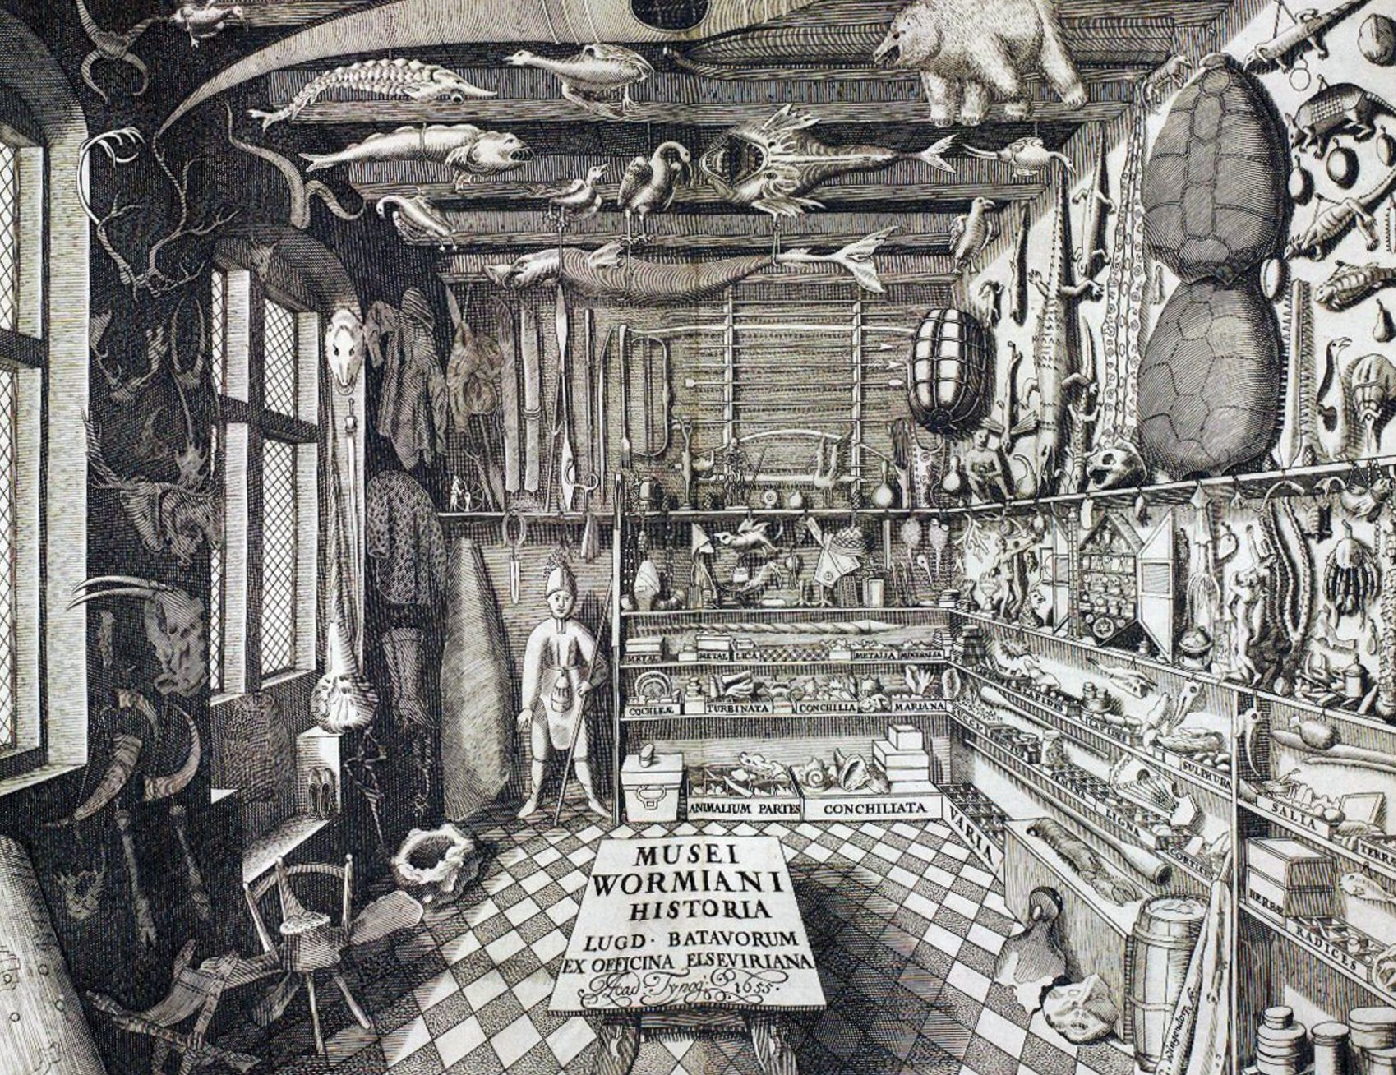
\includegraphics[height=\paperheight]{images/cabinet-wonders.pdf}
            };
        \end{tikzpicture}
     \end{frame}
}

%------------------------------------------------

\begin{frame}
\frametitle{Naturalists of 16th and 17th centuries}

\bbi
  \item rise of collections of curiosities (16th-17th centuries)
  \item assembled by naturalists, botanists, entomologists, etc
  \item flowers, animals, minerals, and objects around the world
  \item discovery of ``new'' colors never seen before
  \item a new insect, coral, flower or gem often revealed a new hue
\ei

\end{frame}

%------------------------------------------------

\begin{frame}
\frametitle{Painter's Primaries}

\bbi
  \item Circa 1930 Cennino Cennini published a description of how a painter's 
  work with seven natural colors namely black, red, yellow, green, lime white,
  blue ultramarine and azurite.
  \item Greek texts show awareness and use of subtractive primary mixtures 
  based on red, yellow and blue colorants to ancient painters and dyers.
  \item By 1664 early chemists were studying dyes and pigments in order to 
  improve them.
  \item Efforts motivated by the huge commercial importance of textile 
  manufacture.
\ei

\end{frame}

%------------------------------------------------

\begin{frame}
\begin{center}
\Huge{\hilit{Isaac Newton's Opticks}}
\end{center}
\end{frame}

%------------------------------------------------

\begin{frame}
\frametitle{Newton's Opticks}
\begin{center}
\ig[width=10cm]{images/newton-opticks.pdf}
\end{center}
\end{frame}

%------------------------------------------------

\begin{frame}
\frametitle{Isaac Newton's Opticks}

\bbi
  \item Physiological limits of color vision not understood before 18th c.
  \item Isaac Newton's \textbf{Opticks} published in 1704.
  \item First scientific analysis of color.
  \item Claimed identification of all fundamental colors and \\
  by extension all possible mixed colors.
\ei

\end{frame}

%------------------------------------------------

\begin{frame}
\frametitle{Newton's Experiments}
\begin{center}
\ig[width=10cm]{images/newton-illustration.pdf}

{\scriptsize {\lolit Engraving of Sir Isaac Newton (1642-1727)}}
\end{center}
\end{frame}

%------------------------------------------------

\begin{frame}
\frametitle{Newton's Experiments}

\bbi
  \item Newton passed sunlight through a triangular prism.
  \item Decomposed light into a rainbow of colors.
  \item Showed that the colors of the rainbow could not be further decomposed.
  \item This experiment marked the beginning of the study of visible light.
\ei

\end{frame}

%------------------------------------------------

{ % all template changes are local to this group.
    \begin{frame}[plain]
        \begin{tikzpicture}[remember picture,overlay]
            \node[at=(current page.center)] {
                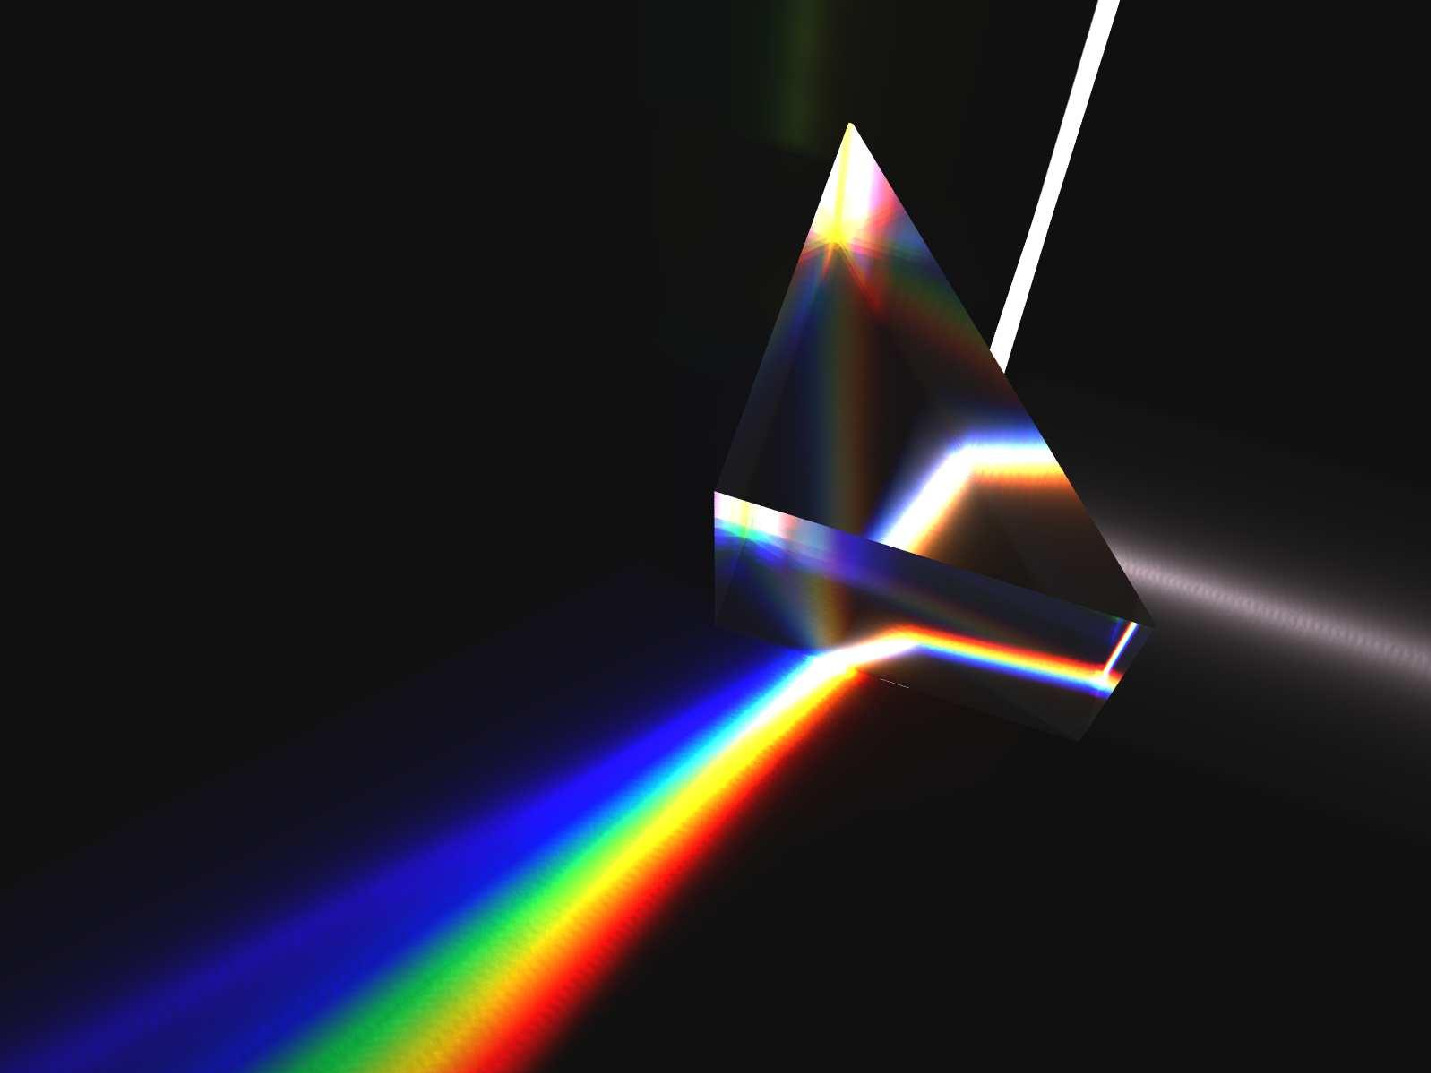
\includegraphics[height=\paperheight]{images/light-prism.pdf}
            };
        \end{tikzpicture}
     \end{frame}
}

%------------------------------------------------

\begin{frame}
\frametitle{Newton's Experiments}

\bbi
  \item Newton claimed to see the seven colors:
  \item red, orange, yellow, green, blue, indigo, and violet.
  \item It is beleived that Newton chose to have 7 colors to parallel the 7
  notes of the standard musical scale.
  \item In practice, 4 or 6 are more natural numbers of colors.
\ei

\end{frame}

%------------------------------------------------

\begin{frame}
\frametitle{Newton's Hue Circle}
\begin{center}
\ig[width=9cm]{images/newton-wheel.pdf}
\end{center}
\end{frame}

%------------------------------------------------

\begin{frame}
\frametitle{Newton's Conclusions}

\bbi
  \item Newton concluded that the color of paints arises from the selective 
  absorption of some spectral hues and the reflection of others.
  \item He rejected the ancient Greek theory that colors arise from 
  mixtures of light and dark.
  \item He rejected the painter's theory that there were just three 
  primary colors---red, yellow and blue.
\ei

\end{frame}

%------------------------------------------------

\begin{frame}
\frametitle{Color Light}

\bbi
  \item Physically, a given color can be related to wavelength.
  \item However, wavelengths do not entirely correspond to the way we perceive
  color.
  \item In terms of wavelength, red and violet are the two most different 
  visible colors.
  \item However, we perceive red and violet as similar or somehow related.
  \item Newton noticed this and arranged the visible colors into a color wheel.
\ei

\end{frame}

%------------------------------------------------

\begin{frame}
\begin{center}
\Huge{\hilit{Color Atlas}}
\end{center}
\end{frame}

%------------------------------------------------

\begin{frame}
\frametitle{Color Systems}

\bbi
  \item 18th century color enthusiasts focused on a specific practical problem:
  \item how to define and represent all possible colors as a single color order system.
  \item These early color models were motivated by a scientific interest in summarizing color perception
  \item by the need for a standardized system of color identification for use in science and industry.
  \item and by an artist's mystical enthusiasm for color.
\ei

\end{frame}

%------------------------------------------------

\begin{frame}
\frametitle{Color Models Requirements}

\bbi
  \item a color specification that defines all possible colors as a mixture of
  fundamental attributes, such as ``primary'' colors;
  \item a geometrical framework that locates all colors in relation to each 
  other and to the fundamental attributes;
  \item a standardized system of unique color labels;
  \item pigment mixture recipes or physical color exemplars
\ei

\end{frame}

%------------------------------------------------

\begin{frame}
\frametitle{Tobias Mayer's Trichromatic Mixing Triangle}
\begin{center}
\ig[height=6cm]{images/mayer-triangle.jpg}

{\small First comprehensive color order system proposed by the Gottingen mathematician and astronomer Tobias Mayer (1723-1762).}
\end{center}
\end{frame}

%------------------------------------------------

\begin{frame}
\frametitle{Color Atlas}

\bbi
  \item Precise spectral mixtures hard to achieve before 19th c.
  \item Naturalists derived color identifications using a color atlas.
  \item A.G. Werner's \textit{Nomenclature of Colors} (1774).
  \item Hand painted colored patches as a visual standard for each color.
\ei

\end{frame}

%------------------------------------------------

\begin{frame}
\frametitle{Nomenclature of Colors}
\begin{center}
\ig[height=8cm]{images/werner-greens.pdf}
\end{center}
\end{frame}

%------------------------------------------------

\begin{frame}
\frametitle{Color Mixture}

\bbi
  \item Recipe of proportional mixture of a few standard colorants.
  \item Industrial color printing by Jakob Christoffel Le Blon.
  \item Multicolor printing system started in 17th century.
  \item Color images created from three primary or "primitive" colored inks.
  \item Modern color mixing systems include the four ink process (CMYK).
\ei

\end{frame}

%------------------------------------------------

\begin{frame}
\frametitle{Runge's Color Sphere}
\begin{center}
\ig[height=8cm]{images/color-sphere.pdf}
\end{center}
\end{frame}

%------------------------------------------------

\begin{frame}
\frametitle{Color Order Systems}

\bbi
  \item Need for a geometrical framework or map of color.
  \item Main idea: colors as combinations of fundamental attributes.
  \item 1st color order system proposed by German astronomer Tobias Mayer 
  in 1758.
  \item \textbf{Color Sphere}: 1st color model to adopt the 3-dimensional 
  framework proposed by German painter Philipp Otto Runge (1810).
  \item Modern color mixing systems include the four ink process (CMYK).
\ei

\end{frame}

%------------------------------------------------

\begin{frame}
\frametitle{Moses Harris's Color Wheel}
\begin{center}
\ig[height=6cm]{images/harris-wheel.pdf}

{\small English entomologist Moses Harris (1731-1785) published a color wheel in his Natural System of Colours (1766)}
\end{center}
\end{frame}

%------------------------------------------------

\begin{frame}
\begin{center}
\Huge{\hilit{Light and Color}}
\end{center}
\end{frame}

%------------------------------------------------

\begin{frame}
\frametitle{Newton's Experiments}
\begin{center}
\ig[width=10cm]{images/newton-illustration.pdf}

{\scriptsize {\lolit Engraving of Sir Isaac Newton (1642-1727)}}
\end{center}
\end{frame}

%------------------------------------------------

\begin{frame}
\frametitle{Light Recap}

\bbi
  \item Light is a form of electromagnetic radiation.
  \item Electromagnetic radiations are characterized by their wavelength.
  \item Visible light has wavelengths in a narrow band centered on 600 nanometers.
\ei

\end{frame}

%------------------------------------------------

\begin{frame}
\frametitle{Electromagnetic Spectrum}
\begin{center}
\ig[width=10cm]{images/visible-spectrum.pdf}
\end{center}
\end{frame}

%------------------------------------------------

\begin{frame}
\frametitle{Visible Light}

\bb{Visible Spectrum}
If the electromagnetic spectrum spanned the distance from Los Angeles to New 
York City, the part visible to the human eye would span the width of a dime.
\eb

\end{frame}

%------------------------------------------------

\begin{frame}
\frametitle{Visible Light}

\bi
  \item Our eyes detect wavelengths in a tiny portion of the em spectrum.
  \item We call this the \textit{visible light spectrum}.
  \item We perceive short wavelengths as blue.
  \item We perceive longer wavelengths as red.
  \item We cannot perceive wavelength beyond the limits of the visible spectrum.
  \item Shorter wavelengths of ultraviolet light.
  \item Longer wavelengths of infrarred radiation.
\ei

\end{frame}

%------------------------------------------------

\begin{frame}
\frametitle{Electromagnetic Spectrum}
\begin{center}
\ig[width=9cm]{images/visible-spectrum.jpg}

{\lolit www.astronomersgroup.org/EMspectrum.html}
\end{center}
\end{frame}

%------------------------------------------------

\begin{frame}
\frametitle{Visible Spectrum}
\begin{center}
\ig[width=9cm]{images/spectrum-thirds.pdf}

If the visible spectrum is divided into thirds, the predominant colors are blue, green, and red.
\end{center}
\end{frame}

%------------------------------------------------

\begin{frame}
\frametitle{Some considerations}

\bbi
  \item Color is part of how we sense the world around us.
  \item Light enters the eyes.
  \item It is processed by light receptors (cones and rods).
  \item And sent via the optic nerves to the brain for further processing and
  interpretation.
  \item Light varies in wavelengths, which our eyes and brain interpret as
  varying colors.
\ei

\end{frame}

%------------------------------------------------

\end{document}
